\section{Recursive neural network models}

The models that we study is are centered aronund a recursively applied composition function which is meant to mimic the recursive construction of meanings in formal semantics. In this scheme, pairs of words are merged into phrase representations by a function that maps from representations of length $2N$ to representations of length $N$. These phrase representations are then further merged with other words and phrases until the entire phrase or sentence being evaluated is represented in a single vector. This vector is then used as the input to a classifier and used in a supervised learning task.

Borrowing a model directly from the existing literature for this task is impossible since none has been proposed to detect asymmetric relations between phrases. Instead, we build a combination model, depicted in Figure \ref{sample-figure}. The two phrases being compared are built up separately on each side of the tree using the same composition function until they have each been reduced to single vectors. Then, the two phrase vectors are fed into a separate comparison layer that is meant to generate a feature vector capturing the relation between the two phrases. The output of this layer is then given to a softmax classifier, which in turn produces a hypothesized distribution over the seven relations.

For a composition layer, we experiment with both a plain neural network layer function (eq. \ref{rnn}) and the RNTN layer function proposed in \citet{chen2013learning} (eq. \ref{rntn}). A sigmoid nonlinearity (elementwise $\tanh$) is applied to the output of either layer function, following Socher et al.
\begin{gather} \label{rnn}
y_{RNN} = f(\mathbf{M} [\vec{x}^{(l)}; \vec{x}^{(r)}] + b_i)\\ % TODO: Add column vectors?
\label{rntn}
y_{RNTN} = f(\vec{x}^{(l)T} \mathbf{A}^{[1...N]} \vec{x}^{(r)} + \mathbf{B} [\vec{x}^{(l)}; \vec{x}^{(r)}] + \vec{c})
\end{gather} % TODO: Explain third order tensor parameter?

The comparison layer uses the same type of function with different parameters and a different nonlinearity function wrapped around it. Rather than use a $\tanh$ nonlinearity here, I found a substantial improvement in performance by using a rectified linear function for $f_{b}$. In particular, I use the leaky rectified linear function \cite{maasrectifier}: $f_{b}(\vec{x})=\max(\vec{x}, 0) + 0.01\min(\vec{x}, 0)$,  applied elementwise. 

To run the model forward and label a pair of phrases, the structure of the lower layers of the network is assembled so as to mirror the tree structures provided for each phrase. The word vectors are then looked up from the vocabulary matrix $V$ (one of the model parameters), and the composition and comparison functions are used to pass information up the tree and into the classifier at the top. The model is trained using backpropagation through structure  \cite{goller1996learning}, wherein the negative log of the probability assigned to the correct label is taken as a cost function, and the gradient of each parameter with respect to that cost function is computed at each node, with information passing down the tree and into both the function parameters and the vocabulary matrix. Gradients for different instances of the composition function or different instances of a word in the same tree are summed to produce at most a single gradient update per parameter.

\textit{Optimization:} I train the model with stochastic gradient descent (SGD), with gradients pooled from randomly chosen minibatches of 32 training examples, and learning rates computed using AdaGrad \cite{duchi2011adaptive} from a starting rate of 0.2. The parameters (including the vocabulary) are initialized randomly using a uniform distribution over $[-0.1, 0.1]$. % TODO: Update

\begin{figure}
\begin{center}
% \Tree [.{\sc softmax classifier}  [.{\sc comparison layer} [.{\sc \ii{dog} vector from $V$} ] [.{\sc composition layer} [.{\sc composition layer} [.{\sc \ii{very} vector from $V$} ] [.{\sc \ii{big} vector from $V$} ] ] [.{\sc \ii{cat} vector from $V$} ] ] ] ]
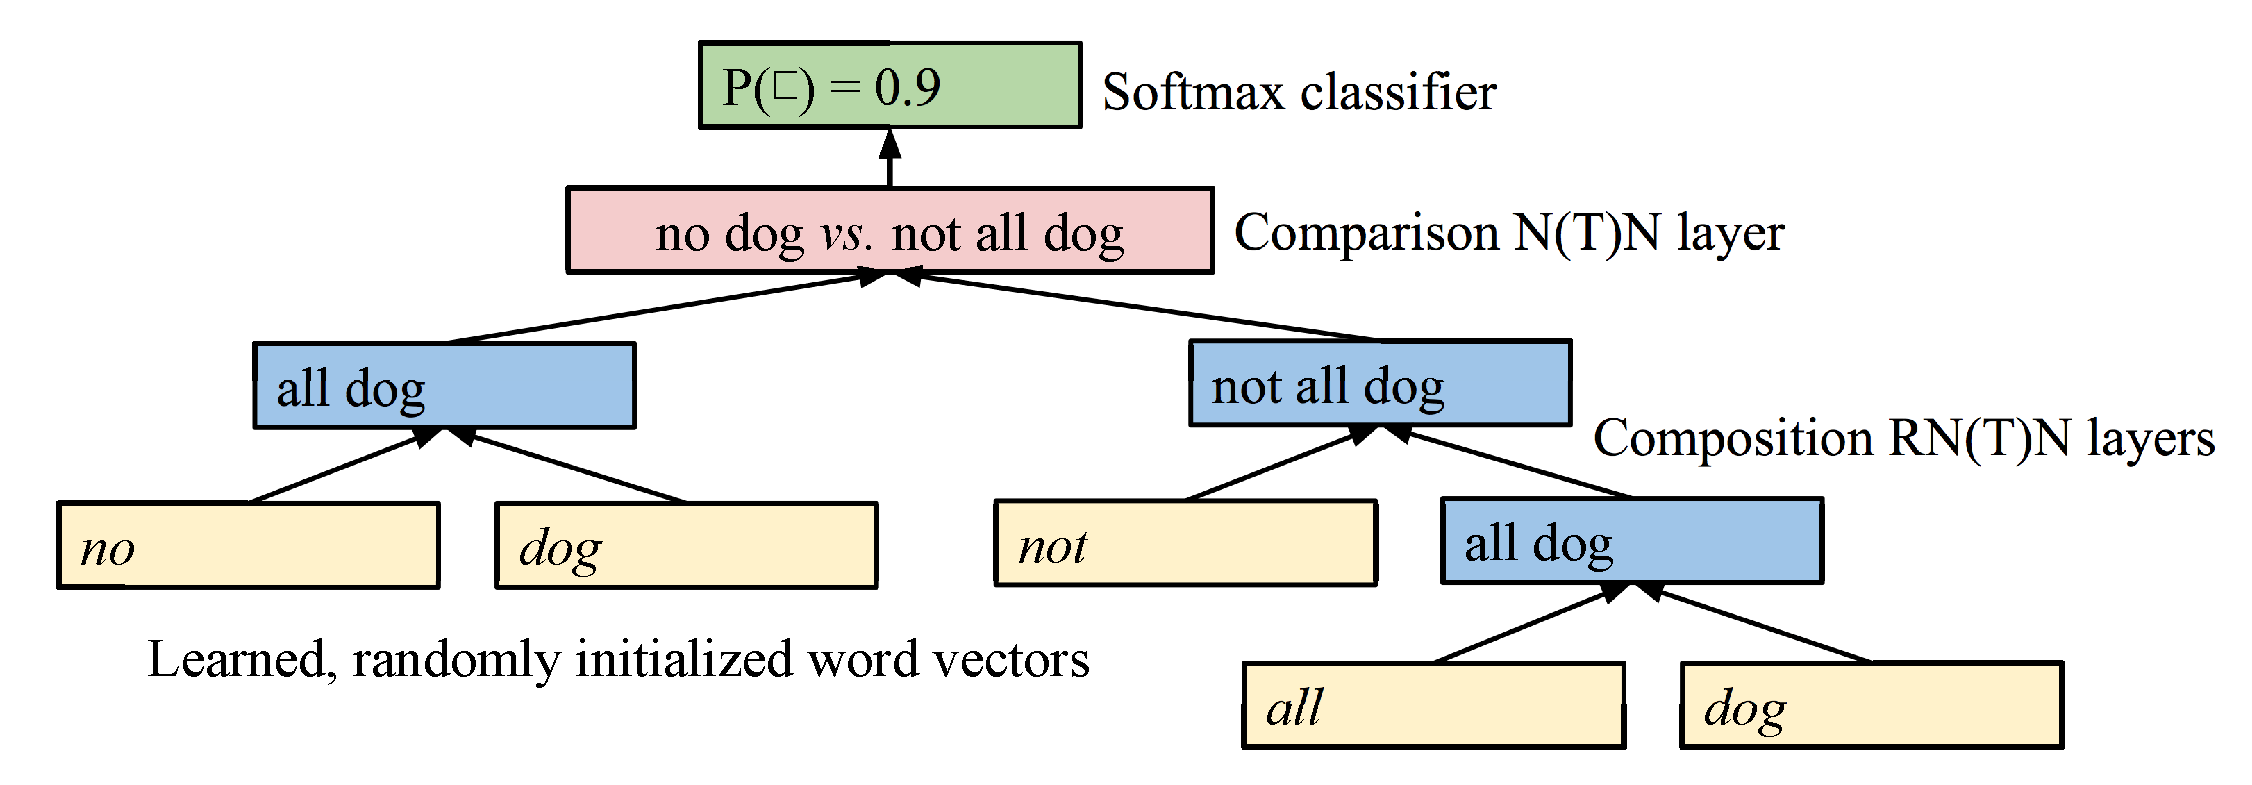
\includegraphics[scale=0.36]{model.eps}
\end{center}
\caption{The model structure used to compare \ii{no dog} and \ii{(not all) dog}. \label{sample-figure}} 
\end{figure} % TODO: Create a more compact figure using something better than qtree.

\ii{Source code and data will be released after the conclusion of the review period.} % TODO: Or upon request? Attach anonymized code?
